\documentclass{article}

\usepackage[margin=3cm]{geometry}

\geometry{a4paper,left=2cm,right=2cm,top=2.54cm,bottom=2.54cm}
%加這個就可以設定字體
\usepackage{fontspec}
    % 普通文字,行距
        \usepackage[onehalfspacing]{setspace}
    
    % 段落間距  (begin doc 才設定)
        \usepackage{parskip}
%使用xeCJK,其他的還有CJK或是xCJK
    % 中文
    \usepackage{xeCJK}
    \setCJKmainfont[AutoFakeBold=3]{DFKai-SB} %设置中
    \usepackage[fontsize=14pt]{fontsize}
% 首行縮排距離
    \setlength\parindent{28pt}
        % 首行縮排
        \usepackage{indentfirst}

%%%%%%%%%%%%%%%%%%%%%%%%
%%%%    三、圖片
%%%%%%%%%%%%%%%%%%%%%%%%


    %%%%    啟用圖片功能
    \usepackage{graphicx}

    %%%%    設定圖片路徑
    \graphicspath{ {./img/} }

    %%%%    設定圖片定位
    \usepackage{float}

    %%%%    把Figure變成"圖"
    \renewcommand{\figurename}{Fig}

%%%%%%%%%%%%%%%%%%%%%%%%
%%%%%%%              end

% 目錄顯示層次
    \setcounter{tocdepth}{2}
% 計算
\usepackage{enumitem}

%設定英文字型,不設的話就會使用預設的字型
\setmainfont{Times New Roman}

\usepackage{fontspec}
\usepackage{titlesec}
\usepackage{graphicx}
\usepackage{physics}
\usepackage{amsmath}
\usepackage{mathtools}
\usepackage{setspace}
\usepackage{subfigure} %所需宏包

\usepackage[hidelinks]{hyperref}
 \usepackage{titlesec}
    % 定义section格式,包括中文数字
   
    \usepackage{zhnumber}
\titleformat{\section}
  {\fontsize{18pt}{15}\bfseries}
  {\selectfont\thesection.}
  {0.5em}
  {}

\usepackage{fancyhdr}
\pagestyle{fancy}

\usepackage{color, xcolor}

\usepackage{algorithm}
\usepackage{algpseudocode}


% New definitions
\algnewcommand\algorithmicswitch{\textbf{switch}}
\algnewcommand\algorithmiccase{\textbf{case}}
\algnewcommand\algorithmicassert{\texttt{assert}}
\algnewcommand\Assert[1]{\State \algorithmicassert(#1)}%
% New "environments"
\algdef{SE}[SWITCH]{Switch}{EndSwitch}[1]{\algorithmicswitch\ #1\ \algorithmicdo}{\algorithmicend\ \algorithmicswitch}%
\algdef{SE}[CASE]{Case}{EndCase}[1]{\algorithmiccase\ #1}{\algorithmicend\ \algorithmiccase}%
\algtext*{EndSwitch}%
\algtext*{EndCase}%

\usepackage{newfloat}
\DeclareFloatingEnvironment[
  fileext = lol ,
  listname = {List Of Listings} ,
  name = Listing
]{listing}

\makeatletter
\newenvironment{breakablealgorithm}
  {% \begin{breakablealgorithm}
    \footnotesize
   \begin{center}
     \refstepcounter{algorithm}% New algorithm
     \hrule height.8pt depth0pt \kern2pt% \@fs@pre for \@fs@ruled
     \renewcommand{\caption}[2][\relax]{% Make a new \caption
       {\raggedright\textbf{\ALG@name~\thealgorithm} ##2\par}%
       \ifx\relax##1\relax % #1 is \relax
         \addcontentsline{loa}{algorithm}{\protect\numberline{\thealgorithm}##2}%
       \else % #1 is not \relax
         \addcontentsline{loa}{algorithm}{\protect\numberline{\thealgorithm}##1}%
       \fi
       \kern2pt\hrule\kern2pt
     }
  }{% \end{breakablealgorithm}
     \kern2pt\hrule\relax% \@fs@post for \@fs@ruled
   \end{center}
  }
\makeatother

\usepackage{pdfpages}
\algnewcommand\And{\textbf{and}}
\algnewcommand\Or{\textbf{or}}

\usepackage{amsmath}

\newcommand\mycommfont[1]{\footnotesize\ttfamily\textcolor{mygreen}{#1}}

\usepackage{tikz, ifthen}
\usetikzlibrary{calc,shapes, positioning,chains,arrows}

\usepackage{everyshi}  % 用于在每一页应用浮水印


% 畫底線
\usepackage{ulem}


\definecolor{myblue}{HTML}{6B73D5}
\definecolor{myred}{HTML}{C00000}
\definecolor{myyellow}{HTML}{FFDB57}

\usepackage[hidelinks]{hyperref}
\hypersetup{urlcolor=myblue, % url
citecolor=black, % citation
linkcolor=black, % table of contents, inner color
colorlinks=true, }
\usepackage{enumitem}

\usepackage{listings}

\definecolor{Blue}{rgb}{0,0,1}
\definecolor{Green}{rgb}{0,0.5,0}
\definecolor{Red}{rgb}{0.64,0.08,0.08}


\lstset{
    captionpos=t,                       % 讓Caption在Bottom的位置
    numbers=left,                       % 程式碼行號
    frame=single,
    showstringspaces=false,             % "不"標註空格
    escapeinside={(*@}{@*)},            % 脫逃字元
    commentstyle=\color{Green},         % Comment顏色
    keywordstyle=\color{Blue},          % Keyword顏色
    stringstyle=\color{Red},            % String顏色
    basicstyle=\ttfamily\scriptsize,         % 字型
    breaklines = true,
}


\begin{document}



\thispagestyle{empty}

\begin{center}
        \vspace*{3cm} %垂直距離
        {\Huge\bf
            \underline{CAD for VLSI Design }\\}%\uppercase\expandafter{\romannumeral 1}}
        \vspace{3cm}
        {\bf\huge Project Assignment 1\\}
        \vspace{0.5cm}
        {\bf\fontsize{23pt}{20}\selectfont Benchmark Translator\\}
        \vspace{4cm}
        {\fontsize{23pt}{26pt} \selectfont Instructor: Andy, Yu-Guang Chen  Ph.D.\\}
        {\fontsize{20pt}{26pt} \selectfont TA: Yi-Ting Lin\\}
        \vspace{2cm}
        \fontsize{22pt}{25pt}\selectfont
        Department/Class: Electrical Engineering 4A\\
        \vspace*{1em}
        Name: {\bf 陳緯亭}\\
        \vspace*{1em}
        Student ID Number: {\bf 109501201}\\
\vspace{2cm}
\end{center}
\newpage


\tableofcontents
\listoflistings


\thispagestyle{empty}
\newpage


 \setcounter{page}{1}

 \lhead{109501201\ 陳緯亭}

% --------------------------------------------------------

\begin{figure}[H]
\flushleft
    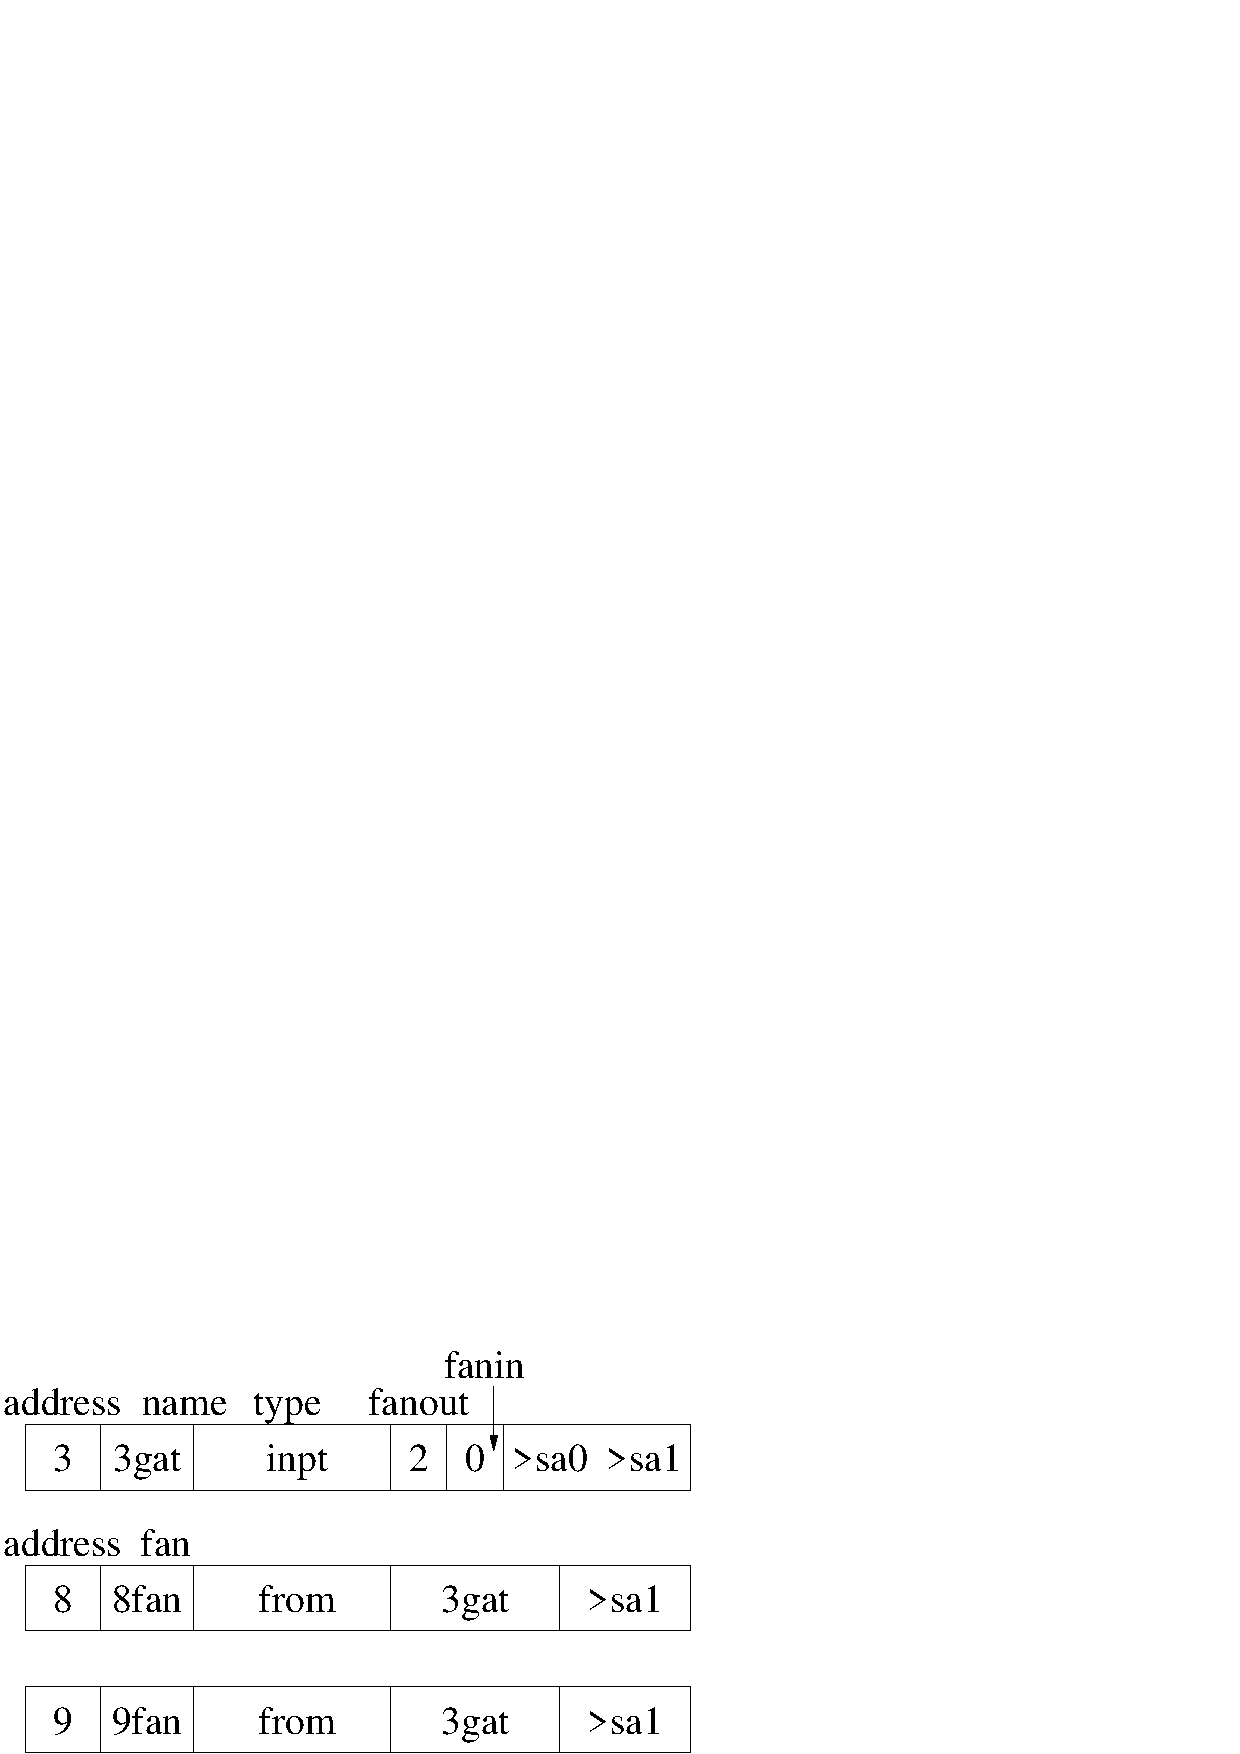
\includegraphics[width=\linewidth]{/Users/chenweiting/Desktop/1.pdf}
\end{figure}

\section{How I compile and execute the program}

\begin{figure}[H]
  \centering
  \includegraphics[width=\linewidth]{./img/2024-03-19-09-22-38.png}
  \caption{Generate an executable file}
  \label{g++}
\end{figure}

\vspace*{-1em}

\begin{figure}[H]
  \centering
  \includegraphics[width=0.5\linewidth]{./img/2024-03-19-09-26-28.png}
  \caption{Use the executable file to ISCAS'85 netlist into Verilog format}
  \label{exe}
\end{figure}

\vspace*{-1em}

\begin{figure}[H]
  \centering
  \includegraphics[width=0.7\linewidth]{./img/2024-03-19-09-30-34.png}
  \caption{Source the following commands}
  \label{source}
\end{figure}

\vspace*{-1em}

\begin{figure}[H]
  \centering
  \includegraphics[width=0.6\linewidth]{./img/2024-03-19-12-45-07.png}
  \caption{Check the correctness}
  \label{check}
\end{figure}

\pagebreak

\section{Pseudo Code}

\begin{figure}[H]
\centering
\includegraphics*[width =0.3 \linewidth]{./1.eps}
\caption{The Variables store the information}
\end{figure}


\begin{breakablealgorithm}
  \caption{Output Algorithm}
  \begin{algorithmic}[1]
    \Function{output\_file}{$vFile$: char*, $c$: PCKT}: \Comment{O($numNode^2*numFanin$)}
  \State ofstream $outFile$($vFile$);
  \State $\textbackslash\textbackslash$ module to $outFile$
  \State $\textbackslash\textbackslash$ input to $outFile$
  \State $\textbackslash\textbackslash$ output to $outFile$
  \State $\textbackslash\textbackslash$ wire to $outFile$
  \For{$i = 0$ to $c \rightarrow numNode$}
      \If{$c \rightarrow nodes[i] \rightarrow type \neq INPT$ and $c \rightarrow nodes[i] \rightarrow type \neq FROM$}
          \State $\textbackslash\textbackslash$ type and instance to $outFile$
          \For{$j = 0$ to $c \rightarrow nodes[i] \rightarrow numFanin$}
              \State $k \gets 0$
              \While{$k < c \rightarrow numNode$}
                  \If{$c \rightarrow nodes[k] \rightarrow address == c \rightarrow nodes[i] \rightarrow fanins[j]$}
                      \State Write ", " + $c \rightarrow nodes[k] \rightarrow outname$ to $outFile$ \Comment{Search form the beginning address.}
                  \EndIf
                  \State $k \gets k + 1$
              \EndWhile
          \EndFor
          \EndIf
  \EndFor
\EndFunction
  \end{algorithmic}
  \end{breakablealgorithm}

  \begin{breakablealgorithm}
    \caption{Second Pass Algorithm}
    \begin{algorithmic}[1]
    \Function{second\_pass}{$inFile$: ifstream, $c$: PCKT}:
        \State string $s$
        \State int $address$, $fanout$, $fanin$
        \State char $name[256]$, $type[256]$
        \State int $col \gets 0$
    
        \While{getline($inFile$, $s$)}
            \State istringstream $iss(s)$
            \If{$s[0] == '*'$}
                \State continue
            \EndIf
            \State $iss \rightarrow$ $address$, $name$, $type$, $fanout$, $fanin$
        \State $\textbackslash\textbackslash$ Get the information from $inFile$ and Store in $c$
    
            \If{fanin $>$ 0}
                \For{$i = 0$ to $fanin$}
                    \State $iss \rightarrow c \rightarrow \text{nodes}[col] \rightarrow \text{fanins}[i]$
                \EndFor
            \EndIf
    
            \If{fanin $\neq$ 0}
                \State $c \rightarrow \text{nodes}[col] \rightarrow \text{type} \gets$ DRIVER
                \State $c \rightarrow \text{nodes}[col] \rightarrow \text{outname} \gets "gat\_out" + address$
                \If{fanout $==$ 0}
                    \State $c \rightarrow \text{nodes}[col] \rightarrow \text{type} \gets$ OUTPT
                \EndIf
            \EndIf
    
            \State $col \gets col + 1$
    
            \If{fanout $>$ 1}
                \For{$i = 0$ to $fanout$}
                    \State getline($inFile$, $s$)
                    \State istringstream $iss(s)$
                    \State $iss \rightarrow address$, $fan$
                    \State $\textbackslash\textbackslash$ Get the information from $inFile$ and Store in $c$
                    \State $col \gets col + 1$
                \EndFor
            \EndIf
    
            \State $c \rightarrow \text{numNode} \gets col$
    
        \EndWhile
    
        \State \Return $c$
    \EndFunction
    \end{algorithmic}
    \end{breakablealgorithm}


\section{PA}

\subsection{The degree of completion of the assignment: \textcolor{red}{ALL}}

\subsection{Code Explanation}

\begin{figure}[H]
\begin{lstlisting}[language = {c++},caption={Preprocessor}, label={library}]
#include <iostream>
#include <string>
#include <fstream>
#include <sstream>
#include <string.h>
\end{lstlisting}
\end{figure}
\vspace*{-1em}

According to \noindent Listing~\ref{func}, there are to structure here to keep all the neccessary circuit information in advantage of facilitate information transfer.


\lstinputlisting[caption={Struct and Function prototype}, label={func}, language={c++}, firstnumber=last]{./Prototype.cpp}

According to \noindent Listing~\ref{main}, I seperate the behavior into two branches - input\_file and output\_file, and then free the memory before the program finish.
 
\lstinputlisting[caption={The main function}, label={main}, language={c++}, firstnumber=last]{./main.cpp}

According to Listing~\ref{inputfile}, the ISCAS'85 format file is read twice. The first time is to collect certain information from the file that will later be used to allocate memory. Subsequently, the information will be thoroughly collected during the second pass. (Note: the file pointer should be moved to the beginning) Since the file name is crucial, as it contains information that will be instantiated as a module with the same name.

\lstinputlisting[caption={Input file process}, label={inputfile}, language={c++}, firstnumber=last]{./input_file.cpp}

According to Listing~\ref{outputfile}, the Verilog file will be generated here. The output stream should begin with the unique module name followed by its port interface list. Subsequently, the output stream should include input signal and output definitions. Next, there should be net type declarations and their instances, followed by output ports and their corresponding input port lists.


\lstinputlisting[caption={Output file process}, label={outputfile}, language={c++}, firstnumber=last]{./output_file.cpp}


According to Listing~\ref{first_pass}, the purpose is to gather preliminary information from the node line to facilitate memory allocation.

\lstinputlisting[caption={First file process}, label={first_pass}, language={c++}, firstnumber=last]{./first_pass.cpp}

According to Listing~\ref{second_pass}, the information should be stored in the structure in this time. To notice that the space should be store the fanin addresses, so it need to be allocate memory. 


\lstinputlisting[caption={Second file process}, label={second_pass}, language={c++}, firstnumber=last]{./second_pass.cpp}

\pagebreak
% ------------------------------
\section{The hardness of this assignment / I overcome it}

\begin{enumerate}
    \item Segmentation fault when writing to a string.\\
    Ans: I change the string to char * in my structure NODE and CKT. Because using string only copy the string object, not the data it holds.
For further information seeing   \href{https://stackoverflow.com/questions/47833332/segmentation-fault-when-using-string-in-structure}{Segmentation fault when using string in structure}


    \item To put const char* into char *, and the data lost.\\
    Ans: Using strdup to keep the data in the structure.
    The usage shown below    \href{https://pubs.opengroup.org/onlinepubs/9699919799/functions/strdup.html}{strdup, strndup - duplicate a specific number of bytes from a string}

    \item Variable names have to start with an alphabetic.\\
    Ans: At the beginning, I only use the node name "1gat" (the second entry on the line) to print out. However, errors like the following occur:

    \href{https://web.stanford.edu/class/ee183/handouts_win2003/VerilogQuickRef.pdf}{Quick
    Reference
    for
    Verilog HDL}

    \begin{figure}[H]
      \centering
    \includegraphics*[width=0.5\linewidth]{./img/2024-03-20-11-09-08.png}
    \end{figure}
    

\end{enumerate}

% ------------------------------

\section{Suggestions}

No.

\end{document}